%杨舒云的实验报告编辑界面,使用了Huanyu Shi,2019级的模板,杨舒云在此拜谢ORZ!

%!TEX program = xelatex
\documentclass[dvipsnames, svgnames,a4paper,11pt]{article}
% ----------------------------------------------------- 
%	加边框的命令
%	参考:https://tex.stackexchange.com/questions/531559/how-to-add-the-page-border-for-first-two-pages-in-latex
\usepackage{tikz}
\usetikzlibrary{calc}
\usepackage{eso-pic}
\AddToShipoutPictureBG{%
\begin{tikzpicture}[overlay,remember picture]
\draw[line width=0.6pt] % 边框粗细
    ($ (current page.north west) + (0.6cm,-0.6cm) $)
    rectangle
    ($ (current page.south east) + (-0.6cm,0.6cm) $); % 边框位置
\end{tikzpicture}}


\usepackage{xcolor}
\definecolor{c1}{HTML}{086173} % 目录颜色 原版为2752C9 紫灰色535AAA 蓝紫色0B0DB7 深蓝色070F94 湖绿色219394 松石灰绿086173
\definecolor{c2}{HTML}{E20129} % 引用颜色 原版\definecolor{c2}{RGB}{190,20,83} 橙色F24729

\usepackage{ctex}
\usepackage[top=28mm,bottom=28mm,left=15mm,right=15mm]{geometry}
\usepackage{hyperref} 
\hypersetup{
	colorlinks,
	linktoc = section, % 超链接位置,选项有section, page, all
	linkcolor = c1, % linkcolor 目录颜色
	citecolor = c1  % citecolor 引用颜色
}
\usepackage{amsmath,enumerate,multirow,float}
\usepackage{tabularx}
\usepackage{tabu}
\usepackage{subfig}
\usepackage{fancyhdr}
\usepackage{graphicx}
\usepackage{wrapfig}  
\usepackage{physics}
\usepackage{appendix}
\usepackage{amsfonts}

%
\usepackage{tcolorbox}
\tcbuselibrary{skins,breakable}
\newtcolorbox{tbox}[2][]{
    colframe=black!70!,
    breakable,
    enhanced,
	boxrule =0.5pt,
    title = {#2},
    fonttitle = \large\kaishu\bfseries,
	drop fuzzy shadow,
    #1
}
\newtcolorbox[auto counter,number within=section]{question}[1][]{
  top=2pt,bottom=2pt,arc=1mm,
  boxrule=0.5pt,
%   frame hidden,
  breakable,
  enhanced, %跨页后不会显示下边框
  coltitle=c1!80!gray,
  colframe=c1,
  colback=c1!3!white,
  drop fuzzy shadow,
  title={思考题~\thetcbcounter:\quad},
  fonttitle=\bfseries,
  attach title to upper,
  #1
}

% ---------------------------------------------------------------------
%	利用cleveref改变引用格式,\cref是引用命令
\usepackage{cleveref}
\crefformat{figure}{#2{\textcolor{c2}{Figure #1}}#3} % 图片的引用格式
\crefformat{equation}{#2{(\textcolor{c2}{#1})}#3} % 公式的引用格式
\crefformat{table}{#2{\textcolor{c2}{Table #1}}#3} % 表格的引用格式


% ---------------------------------------------------------------------
%	页眉页脚设置
\fancypagestyle{plain}{\pagestyle{fancy}}
\pagestyle{fancy}
\lhead{\kaishu 中山大学物理与天文学院电子技术实验\uppercase\expandafter{\romannumeral1}} % 左边页眉,学院 + 课程
\rhead{\kaishu 实验报告By杨舒云\&戴鹏辉} % 右边页眉,实验报告标题
\cfoot{\thepage} % 页脚,中间添加页码


% ---------------------------------------------------------------------
%	对目录、章节标题的设置
\renewcommand{\contentsname}{\centerline{\huge 目录}}
\usepackage{titlesec}
\usepackage{titletoc}
% \titleformat{章节}[形状]{格式}{标题序号}{序号与标题间距}{标题前命令}[标题后命令]
\titleformat{\section}{\centering\LARGE\songti}{}{1em}{}

% ---------------------------------------------------------------------
%   listing代码环境设置
\usepackage{listings}
\lstloadlanguages{python}
\lstdefinestyle{pythonstyle}{
backgroundcolor=\color{gray!5},
language=python,
frameround=tftt,
frame=shadowbox, 
keepspaces=true,
breaklines,
columns=spaceflexible,                   
basicstyle=\ttfamily\small, % 基本文本设置,字体为teletype,大小为scriptsize
keywordstyle=[1]\color{c1}\bfseries, 
keywordstyle=[2]\color{Red!70!black},   
stringstyle=\color{Purple},       
showstringspaces=false,
commentstyle=\ttfamily\scriptsize\color{green!40!black},%注释文本设置,字体为sf,大小为smaller
tabsize=2,
morekeywords={as},
morekeywords=[2]{np, plt, sp},
numbers=left, % 代码行数
numberstyle=\it\tiny\color{gray}, % 代码行数的数字字体设置
stepnumber=1,
rulesepcolor=\color{gray!30!white}
}




% ---------------------------------------------------------------------
%	其他设置
\def\degree{${}^{\circ}$} % 角度
\graphicspath{{./images/}} % 插入图片的相对路径
\allowdisplaybreaks[4]  %允许公式跨页 
\usepackage{lipsum}
\usepackage{adjustbox}
%\usepackage{mathrsfs} % 字体
\captionsetup[figure]{name=Figure} % 图片形式
\captionsetup[table]{name=Table} % 表格形式

\begin{document}
	
	
	
	% 实验报告封面	
	
	% 顶栏
	\begin{table}
		\renewcommand\arraystretch{1.7}
		\begin{tabularx}{\textwidth}{
				|X|X|X|X
				|X|X|X|X|}
			\hline
			\multicolumn{2}{|c|}{预习报告}&\multicolumn{2}{|c|}{实验记录}&\multicolumn{2}{|c|}{分析讨论}&\multicolumn{2}{|c|}{总成绩}\\
			\hline
			\LARGE25 & & \LARGE25 & & \LARGE30 & & \LARGE80 & \\
			\hline
		\end{tabularx}
	\end{table}
	% ---
	
	% 信息栏
	\begin{table}
		\renewcommand\arraystretch{1.7}
		\begin{tabularx}{\textwidth}{|X|X|X|X|}
			\hline
			年级、专业: & 2022级 物理学 &组号: & E2\\
			\hline
			姓名: & 戴鹏辉、杨舒云  & 学号: & 22344016、22344020\\
			\hline
			实验时间: & 2024/4/10 & 教师签名: & \\
			\hline
		\end{tabularx}
	\end{table}
	% ---
	
	% 大标题
	\begin{center}
		\LARGE ET1-6 \quad R、L、C元件阻抗特性研究
	\end{center}
	% ---
	
	% 注意事项
	
	% 基本
	\textbf{【实验报告注意事项】}
	\begin{enumerate}
		\item 实验报告由三部分组成:
		\begin{enumerate}
			\item 预习报告:课前认真研读实验讲义,弄清实验原理;实验所需的仪器设备、用具及其使用、完成课前预习思考题;了解实验需要测量的物理量,并根据要求提前准备实验记录表格(可以参考实验报告模板,可以打印)。\textcolor{red}{\textbf{(20分)}}
			\item 实验记录:认真、客观记录实验条件、实验过程中的现象以及数据。实验记录请用珠笔或者钢笔书写并签名(\textcolor{red}{\textbf{用铅笔记录的被认为无效}})。\textcolor{red}{\textbf{保持原始记录,包括写错删除部分,如因误记需要修改记录,必须按规范修改。}}(不得输入电脑打印,但可扫描手记后打印扫描件);离开前请实验教师检查记录并签名。\textcolor{red}{\textbf{(30分)}}
			\item 数据处理及分析讨论:处理实验原始数据(学习仪器使用类型的实验除外),对数据的可靠性和合理性进行分析;按规范呈现数据和结果(图、表),包括数据、图表按顺序编号及其引用;分析物理现象(含回答实验思考题,写出问题思考过程,必要时按规范引用数据);最后得出结论。\textcolor{red}{\textbf{(30分)}}
		\end{enumerate}
		\textbf{实验报告就是将预习报告、实验记录、和数据处理与分析合起来,加上本页封面。\textcolor{red}{(80分)}}
		\item 每次完成实验后的一周内交\textbf{实验报告}(特殊情况不能超过两周)。
		\item \textbf{其它注意事项}:
		\begin{enumerate}
			\item 请认真查看并理解实验讲义第一章内容;
			\item 注意实验器材的合理使用;
			\item 使用结束使用各种仪器之后需要将其放回原位。
		\end{enumerate}
	\end{enumerate}
	
	% 安全
	\textbf{【实验安全注意事项】}	
	\begin{enumerate}
		\item 采用万用表交流电压档测量交流电压时,请注意有效频率范围。
		\item 在使用示波器测量电压或相位差时,注意示波器两个通道输入信号的接地点接法必须保证信号源、示波器所有通道的接地点接在电路的同一个点上。
		\item 在使用示波器测量电压或相位差时,示波器输入信号的耦合方式要选择交流耦合。
		\item 绘制幅频特性和相频特性曲线时,频率轴采用对数坐标。
		\item 在计算时请注意角频率与频率的转换。
		
	\end{enumerate}
	
	% ---
	
	% 特别鸣谢
	\textbf{【特别鸣谢及模板说明】}	
	
	感谢2019级学长石寰宇为本实验报告提供\LaTeX 模板。\textcolor{red}{\textbf{由于原实验报告模板缺少实验编号,为方便在电脑上整理,故添加自命名编号}}
	% ---
	
	
	
	% 目录
	\clearpage
	\tableofcontents
	\clearpage
	% ---
	
	
	
	% 预习报告	
	
	% 小标题
	\setcounter{section}{0}
	\section{ETX 实验名称××× \quad\heiti 预习报告}
	% ---
	
	% 实验目的
	% \subsection{实验目的}
	\begin{enumerate}
		\item 测量电阻、感抗、容抗与频率的关系,测定$R$-$f$、$X_L$-$f$及$X_c$-$f$特性曲线。
		\item 观察并了解$R$、$L$、$C$元件两端电压与电流间的相位关系。
		
	\end{enumerate}
	% ---
	
	% 仪器用具
	% \subsection{仪器用具}
	\begin{table}[htbp]
		\centering
		\renewcommand\arraystretch{1.6}
		% \setlength{\tabcolsep}{10mm}
		\begin{tabular}{p{0.05\textwidth}|p{0.20\textwidth}|p{0.05\textwidth}|p{0.5\textwidth}}
			\hline
			编号& 仪器用具名称 & 数量 &  主要参数(型号,测量范围,测量精度等) \\
			\hline
			1&  电路原理箱或板& 1 &  \\
			\hline
			2&  函数信号发生器& 1 &  \\
			\hline
			3&  交流毫伏表& 1 &  \\
			\hline
			4&  直流电压表或万用表& 1 & 0~30V \\
			\hline
			5&  2号实验导线& N & 二端2号镀金插头 \\
			\hline
		\end{tabular}
	\end{table}
	% ---
	
	% 原理概述
	% \subsection{原理概述}


	
	
	\clearpage
	% 实验前思考题
	\subsection{实验预习题}
	

		% 思考题1
		\begin{question}
			半导体 PN 节的单向导电原理;
		\end{question}

		半导体 PN 节的单向导电原理,是由于PN结形成时,P区和N区之间形成了一个电场,在没有外加电压时,这个电场会阻止电子和空穴的自由扩散。当施加一个与内建电场方向相同的正向偏置电压时,会使内建电场减弱,电子和空穴能够克服电场的作用而通过PN结,此时会有电流流过,这种状态称为正向导通;
		
		反之,当施加一个与内建电场方向相反的反向偏置电压时,会增强内建电场的作用,阻止电子和空穴通过PN结,此时几乎没有电流通过,称为反向截止。
		
		这种单向导电的原理使得PN结能够作为二极管等器件的基础,实现了电流的控制和单向导电的功能。


		% 思考题2
		\begin{question}
			二极管的大信号模型和小信号模型; 思考如何测量其小信号模型?设计出电路图,实验过程中搭建电路。根据测量出来的二极管伏安特性曲线选择不同正向电流尝试测量不同电流情况下的交流电阻的测量。
		\end{question}

		二极管的大信号模型和小信号模型描述了二极管在不同工作条件下的行为。大信号模型通常用于描述二极管在直流工作条件下的特性,而小信号模型则用于描述二极管在交流工作条件下的特性。

		\begin{enumerate}
			\item 大信号模型:当二极管正向电压比较大的情况下,根据系统计算精度的要求,可以把二极管简化为下列大信号模型中的一种,如\cref{fig:graph1-1}。这几种模型可用于二极管整流电路、钳位电路的近似分析与估算。
			
			% \begin{figure}[htbp]
			% 	\centering
			% 	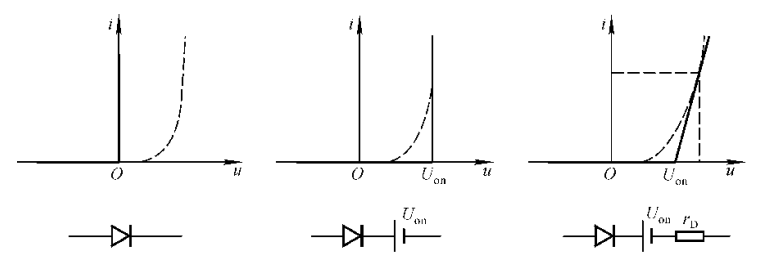
\includegraphics[width=0.7\textwidth]{graph1-1.png}
			% 	\caption{二极管大信号模型}
			% 	\label{fig:graph1-1}
			% \end{figure}

			\item 小信号模型:在小信号模型中,二极管被建模为一个电阻,这个电阻表示二极管的动态电阻,即在交流信号下二极管的电阻值,如\cref{fig:graph1-2}。小信号模型通常用于分析二极管在高频或交流信号下的响应特性。
			
			% \begin{figure}[htbp]
			% 	\centering
			% 	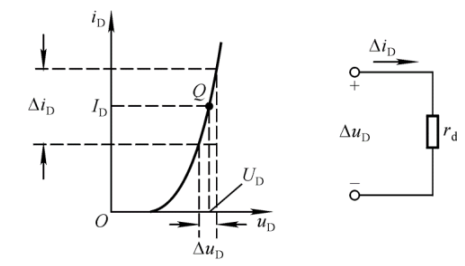
\includegraphics[width=0.5\textwidth]{graph1-2.png}
			% 	\caption{二极管小信号模型}
			% 	\label{fig:graph1-2}
			% \end{figure}

		\end{enumerate}

		为了测量二极管的小信号模型,可以设计一个简单的电路如\cref{fig:graph1-3}

		\begin{figure}[htbp]
			\centering
			\subfloat[二极管大信号模型]
			{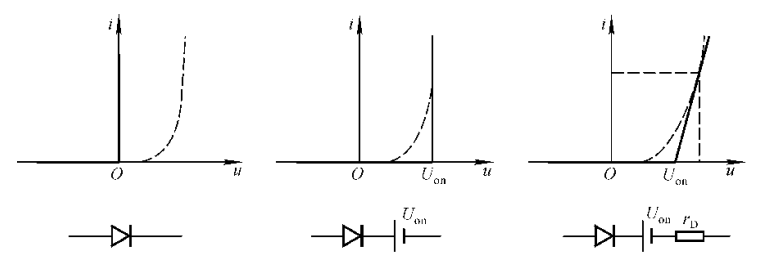
\includegraphics[width=0.7\textwidth]{graph1-1.png}\label{fig:graph1-1}}
			\quad
			\subfloat[二极管小信号模型]
			{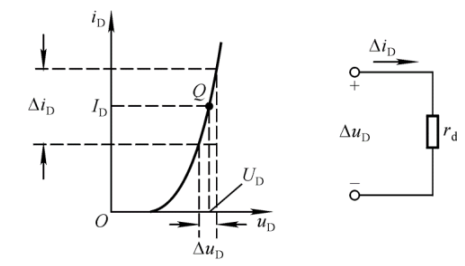
\includegraphics[width=0.31\textwidth]{graph1-2.png}\label{fig:graph1-2}}
			\quad
			\subfloat[二极管小信号模型测试电路]
			{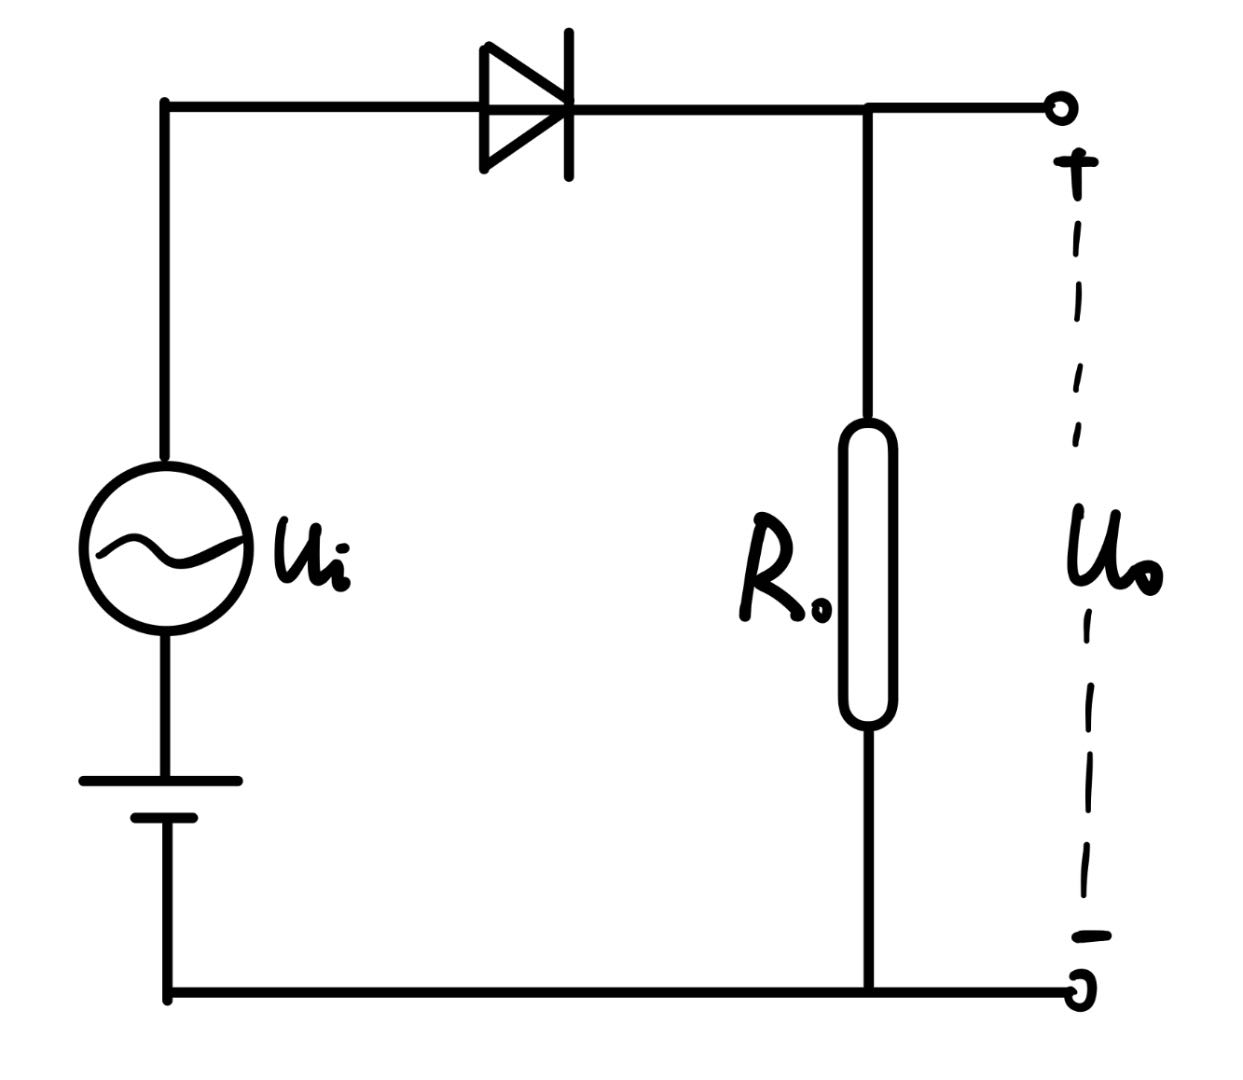
\includegraphics[width=0.31\textwidth]{graph1-3.jpg}\label{fig:graph1-3}}
			\quad

			% \caption{慧差实验结果图}
			\label{fig:graph1}
		\end{figure}


		% \begin{figure}[htbp]
		% 	\centering
		% 	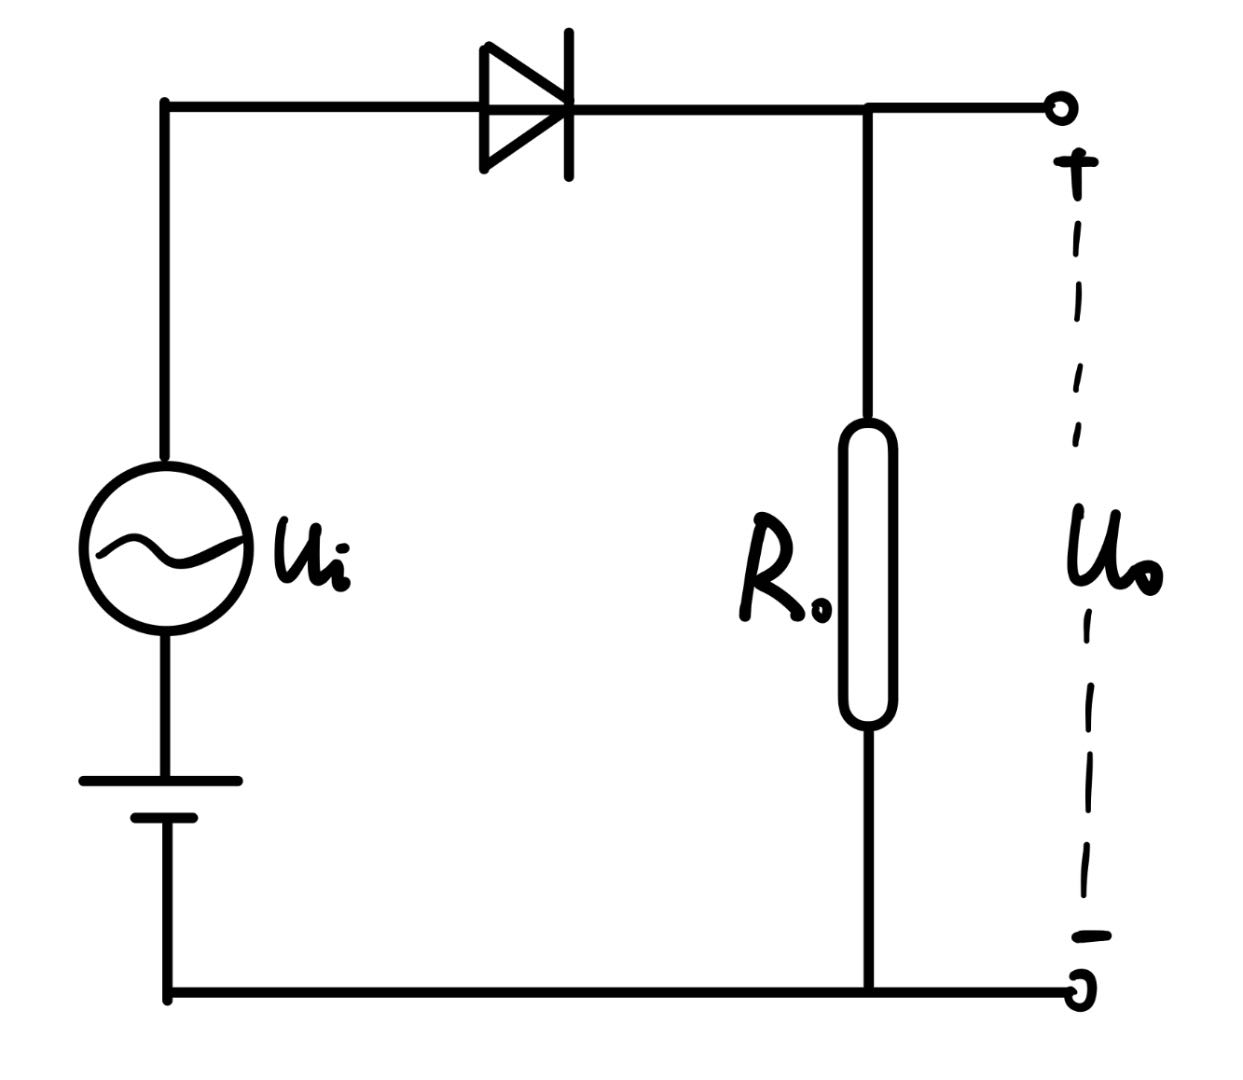
\includegraphics[width=0.4\textwidth]{graph1-3.jpg}
		% 	\caption{二极管小信号模型测试电路}
		% 	\label{fig:graph1-3}
		% \end{figure}

		实验步骤如下:

		\begin{enumerate}
			\item 搭建电路,包括二极管、直流电源、信号发生器和示波器。
			\item 设置直流电压,使二极管正常工作。
			\item 在正向电流的基础上,叠加一个小幅度的正弦交流信号。
			\item 使用示波器测量二极管两端的交流电压和交流电流。
			\item 计算交流电阻,即交流电压与电流的比值。
			
		\end{enumerate}

		
		根据测量出来的二极管伏安特性曲线选择不同正向电流尝试测量不同电流情况下的交流电阻的测量,可以根据需要选择不同的正向电流值进行测量,以了解二极管在不同工作点下的交流电阻特性。



		
		% 思考题3
		\begin{question}
			三极管三种工作状态的条件和特性;
		\end{question}
		
		
		三极管(双极型晶体管)的三种工作状态分别是饱和状态、截止状态和放大状态。这些状态取决于基极(B)、发射极(E)和集电极(C)之间的电压和电流关系。以下是每种状态的条件和特性:

		\begin{enumerate}
			\item 饱和状态:
				\begin{enumerate}
					\item 条件:基极-发射极间的电压$V_{BE}$大于或等于硅管饱和压降(通常为0.7V),集电极-发射极间的电压$V_{CE}$足够小,使得三极管中的所有PN结都处于正向偏置状态。
					\item 特性:三极管处于最低电阻状态,集电极几乎与地电势相接近,输出电压接近零,输出电流最大。在饱和状态下,三极管可以被视为一个开关,完全导通。
				\end{enumerate}
			
			\item 截止状态:
				\begin{enumerate}
					\item 条件:基极-发射极间的电压低于硅管的硅流压降,或者基极没有外加电压;集电极-发射极间的电压足够高,使得所有PN结都处于反向偏置状态。
					\item 特性:三极管处于最高电阻状态,集电极接近电源电压,输出电压接近最大值。在截止状态下,三极管可以被视为一个关闭的开关,完全不导通。
				\end{enumerate}
			
			\item 放大状态:
				\begin{enumerate}
					\item 条件:基极-发射极间的电压大于硅管的硅流压降,且集电极-发射极间的电压足够大,使得三极管工作在放大区。
					\item 特性:三极管的电流增益很大,小信号输入可以得到大信号输出。在放大状态下,三极管被用作放大器的核心部件。
				\end{enumerate}
			
		\end{enumerate}


		三极管的工作状态由其外部电路提供的电压和电流决定。




		% 思考题4
		\begin{question}
			三极管处于的放大和饱和状态时, $V_{CE}$受电路中的哪些因素影响?
		\end{question}

		
		在三极管处于放大和饱和状态时,集电极-发射极间的电压$V_{CE}$受到电路中的以下因素影响:

		\begin{enumerate}
			\item 放大状态下的$V_{CE}$影响因素:
				\begin{enumerate}
					\item 输入信号的幅度和频率:输入信号的幅度和频率会影响三极管的放大倍数,进而影响输出信号的幅度和相位。
					\item 负载电阻:负载电阻的大小会影响集电极电压的稳定性和输出信号的失真程度。
					\item 输入电压:输入信号的大小和极性会直接影响三极管的工作状态和输出信号的波形。
				\end{enumerate}

			\item 饱和状态下的$V_{CE}$影响因素:
				\begin{enumerate}
					\item 基极电压和发射极电流:当基极电压大于或等于硅管饱和压降时,三极管进入饱和状态,此时$V_{CE}$约为几百毫伏,主要取决于集电极电流和负载电流。
					\item 负载电阻:负载电阻的大小会影响$V_{CE}$的稳定性和输出信号的失真程度。
					\item 输入信号的幅度和频率:输入信号的幅度和频率对$V_{CE}$的影响较小,但仍会影响输出信号的质量和失真程度。
				\end{enumerate}

			
		\end{enumerate}



		总的来说,$V_{CE}$受到输入信号、负载电阻和三极管本身的电流和电压特性的影响。在放大状态下,$V_{CE}$主要受到输入信号和负载电阻的影响;在饱和状态下,$V_{CE}$主要受到输入信号、基极电压和负载电阻的影响。

	% ---
	
	
	
	% 实验记录	
	\clearpage
	
	% 顶栏
	\begin{table}
		\renewcommand\arraystretch{1.7}
		\centering
		\begin{tabularx}{\textwidth}{|X|X|X|X|}
			\hline
			专业: & 物理学 & 年级: & 2022级 \\
			\hline
			姓名: & 戴鹏辉 & 学号: & 22344016\\
			\hline
			室温: &  & 实验地点: & A522 \\
			\hline
			学生签名:& 见\textbf{附件}部分 & 评分: &\\
			\hline
			实验时间:& 2024// & 教师签名:&\\
			\hline
		\end{tabularx}
	\end{table}
	% ---
	
	% 小标题
	\section{ET7 半导体器件传输特性研究  \quad\heiti 实验记录}
	% ---
	
	% 实验过程记录
	\subsection{实验内容、步骤与结果}
	
	%
	\subsubsection{操作步骤记录}
	\begin{enumerate}
		\item 
	\end{enumerate}	
	
	%
	\subsubsection{}
	\begin{enumerate}
		\item \begin{table}[h]
			\centering
			\caption{表格示例}
			\label{tab:tab1}
			\begin{tabular}{|c|c|c|c|c|c|}
				\hline
				组1/序号i & 1 & 2 & 3 & 4 & 5 \\
				$v_{1i}(m/s)$ & 1.26 & 1.08 & 1.00 & 0.75 & 0.38 \\
				$f_{1i}(Hz)$ & 40073 & 40127 & 40105 & 40088 & 40066 \\
				\hline
				组2/序号i & 1 & 2 & 3 & 4 & 5 \\
				$v_{2i}(m/s)$ & 1.21 & 1.06 & 0.99 & 0.52 & 0.57 \\
				$f_{2i}(Hz)$ & 40143 & 40125 & 40084 & 40080 & 40067 \\
				\hline
				组3/序号i & 1 & 2 & 3 & 4 & 5 \\
				$v_{3i}(m/s)$ & 1.15 & 0.98 & 0.78 & 0.59 & 0.36 \\
				$f_{3i}(Hz)$ & 40135 & 40115 & 40092 & 40070 & 40044 \\
				\hline
			\end{tabular}
		\end{table}		
	\end{enumerate}
	
	% ---
	
	% 原始数据
	\clearpage
	\subsection{原始数据记录}
	实验记录本上的原始数据见%\cref{}(签字)。
	
	实验台桌面整理见%\textbf{附件}部分(\cref{})。
	
	其它原始数据见%\cref{}。
	% ---
	
	% 问题记录
	\subsection{实验过程遇到问题及解决办法}
	\begin{enumerate}
		\item 
	\end{enumerate}
	% ---
	
	
	
	% 分析与讨论	
	\clearpage
	
	% 顶栏
	\begin{table}
		\renewcommand\arraystretch{1.7}
		\begin{tabularx}{\textwidth}{|X|X|X|X|}
			\hline
			专业:& 物理学 &年级:& 2022级\\
			\hline
			姓名: & 戴鹏辉 & 学号:& 22344016\\
			\hline
			日期:& 2023/11/23 & 评分: &\\
			\hline
		\end{tabularx}
	\end{table}
	% ---
	
	% 小标题
	\section{ETX 实验名称××× \quad\heiti 分析与讨论}
	% ---
	
	% 数据处理
	\subsection{实验数据分析}
	
	%
	\subsubsection{}
	\begin{enumerate}
		\item 
	\end{enumerate}
	
	%
	\subsubsection{}
	\begin{enumerate}
		\item 
	\end{enumerate}
	
	%
	\subsubsection{}
	
	% ---
	
	% 实验后思考题
	\subsection{实验后思考题}
	
	%思考题1
	\begin{question}
		
	\end{question}
	
	% 思考题2
	\begin{question}
		
	\end{question}
	
	% 思考题3
	\begin{question}
		
	\end{question}
	
	% ---
	
	
	% 结语部分
	\clearpage
	
	% 小标题
	\section{ETX 实验名称××× \quad\heiti 结语}
	% ---
	
	% 总结、杂谈与致谢
	\subsection{实验心得和体会、意见建议等}
	\begin{enumerate}
		\item 
	\end{enumerate}
	% ---
	
	% 参考文献
	\subsection{参考文献}
	[1] 维基百科 https://zh.wikipedia.org
	
	[2] 沈韩.基础物理实验.——北京:科学出版社,2015.2 ISBN:978-7-03-043311-4
	
	% ---
	
	% 附件
	\subsection{附件及实验相关的软硬件资料等}
	试验台桌面整理如%\cref{}所示。
	
	实验报告个人签名如\cref{fig:name}。
	
	\begin{figure}[htbp]
		\centering
		
\includegraphics[width=0.7\textwidth]{name.png}
		\caption{个人签名}
		\label{fig:name}
	\end{figure}
	
	% ---
	
	相关代码已上传至Github。
	
	
	
\end{document}